\begin{comment}
\yanlin{
TODOs:
\begin{itemize}
\item UML Diagram for full solution in introduction with informal explanation
\item Move Figure 5 to end of Section 2 together with explanation
\item Improve Figure 5 with additional mbody calls
\item Improve Figure 5 with visual information that signals that in examples d) and e) then D does not type-check
\item Make names of classes more consistent in Figure 5
\item Add example (f) : A m      B m   C m   D  m  This would compile, note that if it was BArrowA m and/or CArrowA m it would also compile and D would have the same observable behaviour
\item remove S1 “Unfortunately, such an issue ...”
\item (\checkmark)S2, should remove the discussion about JFrmae. all return type void.
\item (\checkmark)S2, mention DrawableDeck in P2.3 is a new version of DrawableDeck before.
\item (\checkmark)S2, “Ideally, we want that invocation to be dynamically dispatched.” --> “In FHJ, this invocation is dynamically dispatched.“. and revise the following paragraph on “we may have to copy the shuffleAndDraw code into SafeDeck, so as to be adaptive to the new draw. “.
\item S2.2 revise paragraph “Implicit and Explicit Upcasts “.
\item S2.3 (Maybe) put “Potential solutions/workarounds in existing languages” after “FHJ solution”.
\item S2.3 (Maybe) add “redraw()” method in Drawable. and add another method call similar to shuffleAndDraw()
\item Talk about Fig5 earlier. Move from S4.1 to S2.3 (a peek of ..)
%\item The keywords in code are barely distinghuishable from other code,  make them bolder/darker

\item (\checkmark)in Figure 1, the UML diagram on the right side is not quite right, 
we want to be able to override draw from Drawable in DrawableSafeDeck, 
the override (which is *the most important point*) is not in the UML diagram.
  => Figure 1 on the right is the UML for P3 potential workaround, not for P3 FHJ, we need another UML. 
\item Submit abstract
\item Introduction to revise (by Bruno)
\item Revise overview (Yanlin and Haoyuan)
\item Section 4, 5 (Haoyuan)
\item Section 6 (Yanlin)
\item Section 7 (Yanlin and Haoyuan)
\end{itemize}
}
\end{comment}

\section{Introduction}
Inheritance in Object-Oriented Programming (OOP) offers a mechanism
for code reuse. However many OOP languages are restricted to single
inheritance, which is less expressive and flexible than multiple
inheritance. Nevertheless, different flavours of multiple inheritance
have been adopted in some popular OOP languages. C++ has had 
multiple inheritance from the start. Scala adapts the ideas from traits~\cite{scharli03traits,Ducasse:2006:TMF:1119479.1119483,Liquori08ftj}
and mixins~\cite{bracha90mixin,Flatt1998,van1996encapsulation,Ancona2003,Hendler86} to offer a disciplined form of multiple inheritance. Java 8 
offers a simple variant of traits, disguised of interfaces with default methods~\cite{goetz12fdefenders}.

A reason why programming languages have resisted to multiple
inheritance in the past is that, as Cook~\cite{Cook1987} puts it, 
``\emph{multiple inheritance is good but there is no good way to do it}''.
One of the most sensitive and critical issues is perhaps the ambiguity
introduced by multiple inheritance. One case is the famous
\textit{diamond problem}~\cite{Sak89dis,Singh1995} (also known as ``fork-join inheritance''~\cite{Sak89dis}). 
In the diamond problem, inheritance allows
one feature to be inherited from multiple parent classes that share a
common ancestor. Hence
conflicts arise. The variety of strategies for resolving such conflicts
urges the occurrence of different multiple inheritance models,
including traits, mixins, CZ~\cite{malayeri2009cz}, and many others. Existing
languages and research have addressed the issue of diamond inheritance extensively. Other issues
including how multiple inheritance deals with state, 
have also been discussed quite extensively~\cite{classless,malayeri2009cz,stroustrup1995}.

In contrast to diamond inheritance, the second case of ambiguity
is \textit{unintentional method conflicts}~\cite{scharli03traits}. In
such a case conflicting 
methods do not actually refer to the same feature. 
In a nominal system, methods can be designed for different
functionality, but happen to have the same names (and signatures).
A simple example of this situation is two \lstinline{draw} methods that
are inherited from a deck of cards and a drawable widget. 
In such context, the two \lstinline{draw} methods have very different meanings, 
but they happen to share the same name.
%%This issue was proposed by the trait paper, so-called
When inheritance is used to compose these methods, a compilation 
error happens due to conflicts. However, unlike the diamond problem,
the conflicting methods have very different meanings and do not share a
common parent. We call such a case \textit{triangle inheritance}, in
analogy to diamond inheritance.

%Unintentional method conflicts are perhaps less common than the diamond
%problem. 

When unintentional method conflicts happen, they can have severe
effects in practice if no
appropriate mechanisms to deal with them are available. 
% Unfortunately, such an issue has not received much formal study 
% before. 
In practice, existing languages only provide limited support for
the issue. In most languages, the mechanisms available to deal with this problem are the same as the diamond
inheritance. However, this is often inadequate and can lead 
to tricky problems in practice. This is especially the case
when it is necessary to combine two large modules and their features,
but the inheritance is simply prohibited by a small conflict. 
As a workaround from the diamond inheritance side, it is possible to
define a new method in the child class to override those conflicting
methods. However, using one method to fuse two unrelated features
is clearly unsatisfactory. Therefore we need a better solution to keep both
features separately during inheritance, so as not to break
\emph{independent extensibility}~\cite{zenger05independentlyextensible}.

C++ and C\# do allow for two
unintentionally conflicting methods to coexist in a class. C\# allows
this by interface multiple inheritance and explicit method
implementations. But since C\# is a single inheritance language, 
it is only possible to \emph{implement} multiple interfaces (but not
multiple classes). %We will have more detailed discussion on this in Section~\ref{sec:relatedwork}.
C++ accepts triangle inheritance and
resolves the ambiguity by specifying the expected path by
\emph{upcasts}. However, neither the C\# or C++ approaches allow
such conflicting methods to be further overridden. 
% However, C++ has
% limited support for virtual methods with unintentional conflicts, and
% it will often throw errors when composing them. This is again
% unsatisfactory because virtual methods are pervasive in OOP and used 
% for code reuse and extensibility. A problem with the C++ approach is
% that programmers can only use either static or dynamic dispatching separately, but dealing
% with unintentional method conflicts seems to require a combination of
% both. 
Some other workarounds or approaches include delegation and
renaming/exclusion in the trait model. However renaming/exclusion 
can break the subtyping relation between a subclass and its parent.
This is not adequate for the class model commonly used in mainstream 
OOP languages, where the subclass is always expected to be a subtype 
of the parent class. 

%%Yet they still have various
%%drawbacks as we will discuss in Section~\ref{sec:overview}.
% \bruno{The previous paragraph needs to be revised to better discuss the
%   limitations of the C++ approach. Yanlin, Marco can you have a look
%   at this?}


%Having tolerance for unintentional method conflicts does not mean to
%sacrifice extensibility, hence in contrast with static dispatch and
%dynamic dispatch, 

This paper proposes two mechanisms to deal with unintentional method
conflicts: \textit{hierarchical dispatching} and \emph{hierarchical
  overriding}. Hierarchical dispatching is inspired by the mechanisms in C++ and
provides an approach
to method dispatching, which combines static and dynamic
information. Using hierarchical dispatching, the method binder will look
at both the \emph{static type} and the \emph{dynamic type} of the
receiver during runtime. When there are multiple branches that cause
unintentional conflicts, the static type can specify one branch among
them for unambiguity, and the dynamic type helps to find the most
specific implementation. In that case, both unambiguity and
extensibility are preserved. The main novelty over existing work is 
the formalization of the essence of a hierarchical dispatching
algorithm, which (as far as we know) has not been formalized before. 

\begin{figure}[t]
\center  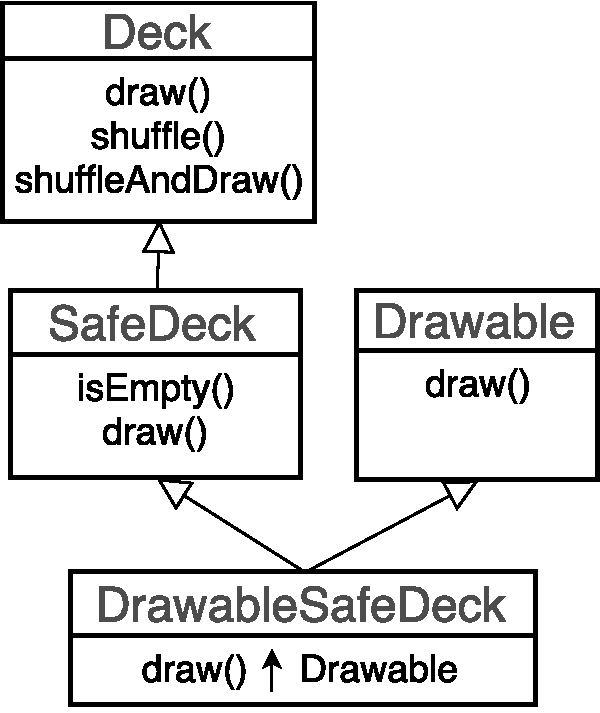
\includegraphics[height=4cm]{pics/DrawableSafeDeck3.pdf}
\caption{\lstinline|DrawableSafeDeck|: an illustration of hierarchical overriding.}
\label{fig:main}
\end{figure}

\textit{Hierarchical overriding} is a novel language
mechanism that allows method overriding to be applied
only to one branch of the class hierarchy. Hierarchical overriding 
adds expressive power that is not available in languages such as 
C++ or C\#. Hierarchical overriding allows overriding to work 
for classes with multiple (conflicting) methods sharing the 
same names and signatures. An example is presented in 
Figure~\ref{fig:main}. In this example, there are 4 classes/interfaces.
Two classes model a deck of cards (\lstinline|Deck|) and a class for
drawable widgets (\lstinline|Drawable|). 
The class \lstinline|SafeDeck| adds functionality to check whether the
deck is empty and to prevent drawing a card from an empty deck. 
The interesting class is \lstinline|DrawableSafeDeck|, which inherits 
from both \lstinline|SafeDeck| and \lstinline|Drawable|. Hierarchical
overriding is used in \lstinline|DrawableSafeDeck| to keep two separate \lstinline|draw|
methods for each parent, but overriding \emph{only} the \lstinline|draw|
method coming from \lstinline|Drawable|, in order to draw a widget
with a deck of cards. Note that hierarchical overriding is denoted in the UML
diagram with the notation
\lstinline|draw()|$\shneg$\lstinline|Drawable|, expressing that the \lstinline|draw| method from \lstinline|Drawable|
is overridden. Although in this example only one of the
\lstinline|draw| methods is overridden (and the other is simply inherited), hierarchical overriding
supports multiple conflicting methods to be independently overridden as well.


To present hierarchical overriding and dispatching, we introduce a
formalized model \MIM{} in Section~\ref{sec:formalization} based on
Featherweight Java~\cite{Igarashi01FJ}, together with theorems and
proofs for type soundness. 
In summary, our contributions are:
\begin{itemize}
	\item \textbf{A formalization of a hierarchical dispatching algorithm} that integrates both the static type and dynamic type for method dispatch, and 
	ensures unambiguity as well as extensibility in the presence
        of unintentional method conflicts.
	\item \textbf{Hierarchical overriding:} a novel notion that allows
          methods to override individual branches of the class hierarchy.
	\item \textbf{\name:} a formalized model based on
          Featherweight Java, supporting the above features. 
          We provide the static and dynamic semantics and prove the
          type soundness of the model.
	\item \textbf{Prototype implementation\footnote{https://github.com/YanlinWang/MIM/tree/master/Calculus}:} a
          simple implementation of \MIM{} interpreter in Scala.
\end{itemize}

 